% Start here


\chapter{Introduction}
\label{sec:intro}

\begin{comment}
MPD : Todo
\end{comment}

 \begin{figure}
  \centering
  \fbox{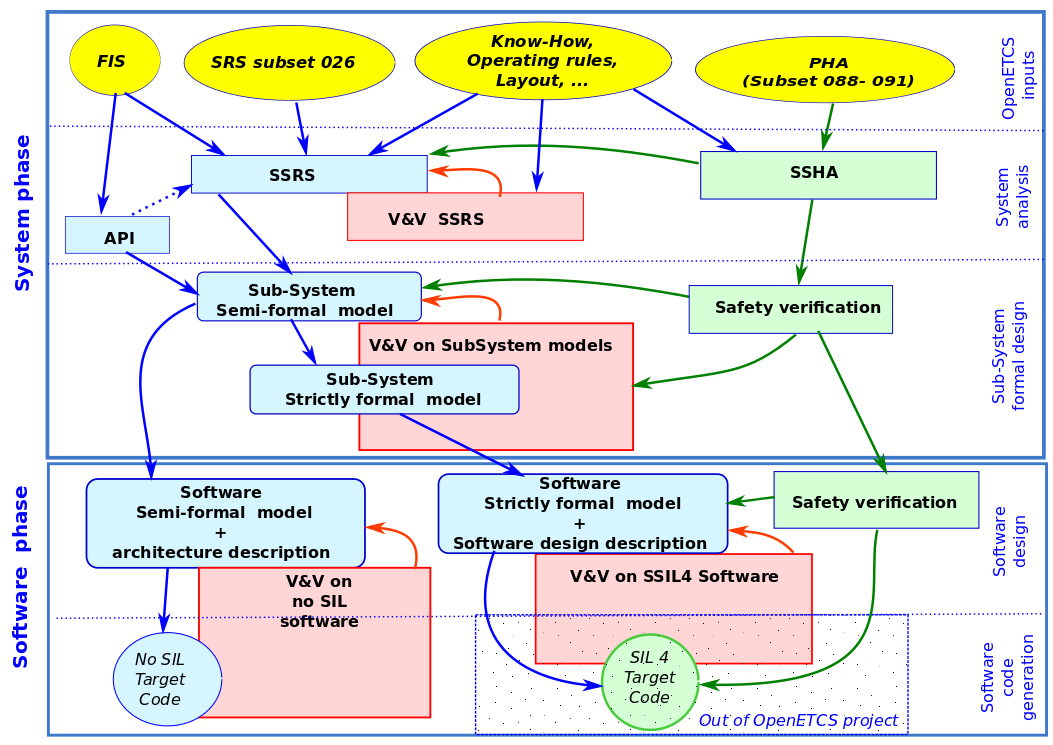
\includegraphics[scale=0.45]{WholeProcess.png}}
  \caption{Main OpenETCS process}
  \label{fig:main_process}
\end{figure}




%%%%%%%%%%%%%%%%%%%%%%%%%%%%%%%%%%%%%%%%%%%%%%%%%%%%%%%%%%%%%%%


\section{Glossary}
\label{sec:glossary}

\begin{description}
\item[API] Application Programming Interface
\item[FME(C)A] Failure Mode Effect (and Criticity) Analysis
\item[FIS] Functional Interface Specification
\item[HW] Hardware
\item[I/O] Input/Output
\item[OBU] On-Board Unit
\item[PHA] Preliminary Hazard Analysis
\item[QA] Quality Analysis
\item[RBC] Radio Block Center
\item[RTM] RunTime Model
\item[SIL] Safety Integrity Level
\item[SRS] System Requirement Specification
\item[SSHA] Sub-System Hazard Analysis
\item[SSRS] Sub-System Requirement Specification
\item[SW] Software
\item[THR] Tolerable Hazard Rate
\item[V\&V] Verification \& Validation
\end{description}

%%%%%%%%%%%%%%%%%%%%%%%%%%%%%%%%%%%%%%%%%%%%%%%%%%%%%%%%%%%%%%%


